%!tex root=./thesis.tex
\chapter{Radio Sources}
\label{cha:background}

    As its title suggests, this thesis is focused on the identification of extended radio sources. This chapter introduces extended radio sources, describing what we see when we look at the sky with radio eyes (and radio telescopes). We will discuss the different kinds of radio sources that we can observe, how they are distributed throughout the universe, and key issues surrounding their identification.

    \begin{figure}[ht]
        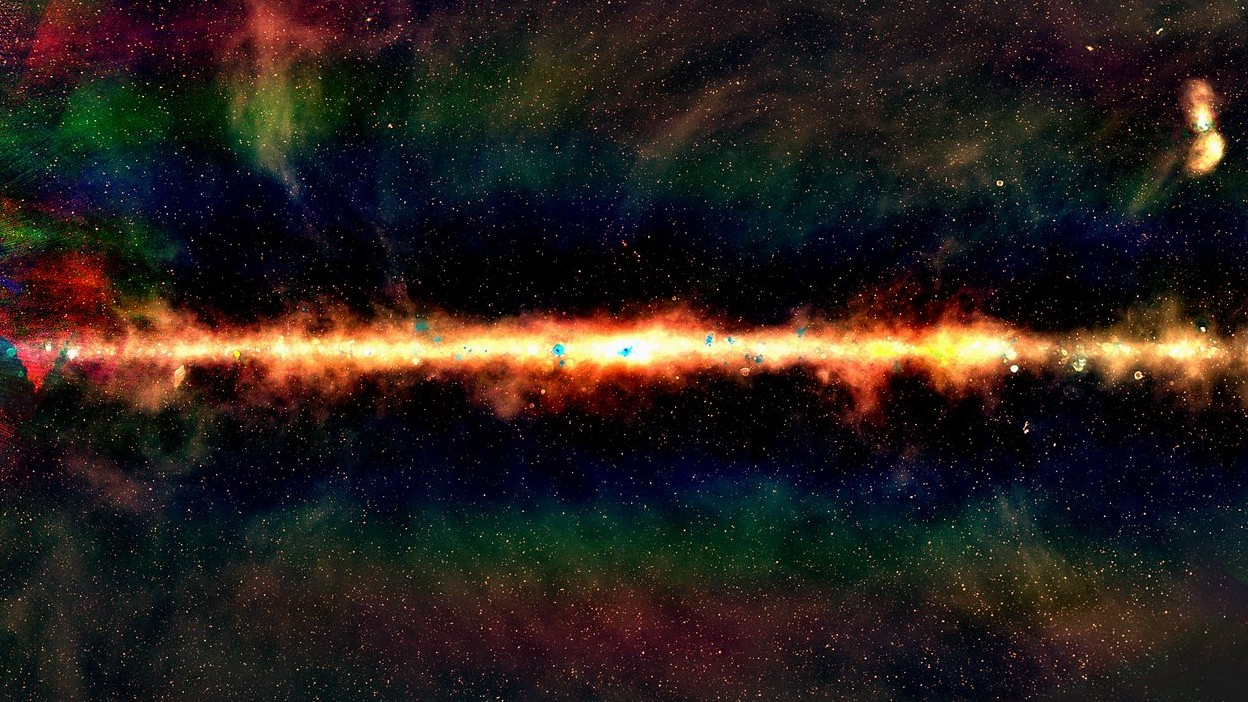
\includegraphics[width=\textwidth]{images/gleam.jpg}
        \caption[False-colour image of the radio sky from the GLEAM survey.]{\label{fig:gleam} False-colour image of the radio sky from the GLEAM survey. (Image: Natasha Hurley-Walker, Curtin University/ICRAR \citeneeded)}
    \end{figure}

\section{The Extragalactic Radio Sky}
\label{sec:extragalactic-radio-sky}

    The extragalactic sky appears quite different at different wavelengths. While an optical observer may look at a distant galaxy and see spirals and halos, an infrared observer will see discs and dust. What does the radio astronomer see? 
    \autoref{fig:gleam} shows a false-colour image of the radio sky. The plane of the Milky Way is clearly visible through the centre, but nearly every other object in this image is a galaxy. These galaxies fall into two main categories: those that emit radio due to star formation (called \defn{star-forming galaxies}), and those that emit radio due to \defn{active galactic nuclei} (AGN; called \defn{radio galaxies} in this thesis).

    Non-AGN emission from distant galaxies traces the recent star-formation rate (SFR). Besides low-power thermal emission, stellar radio emission from galaxies mainly comes from massive ($\gtrapprox 8$ M$_\odot$) stars, through two emission mechanisms. The first is through H~II regions, which are ionised by such stars. The ionised electrons emit bremsstrahlung radiation at radio wavelengths. The second emission mechanism is supernovae. Massive stars may end their lives in Type II and Type Ib supernovae, which can result in supernova remnants. These remnants emit synchrotron radiation. Massive stars like these are short-lived ($\lessapprox 3 \times 10^7$ yr), and the corresponding emitting electrons have similarly short lifetimes ($\lessapprox 10^8$ yr). The radio effects of these stars are therefore also short-lived, which is why radio emission traces the recent SFR \citep{condon_radio_1992}. Star formation-associated emission is mainly found in the disc of spiral galaxies, as this is where the star formation rate is highest. In particular, there is no star-forming radio emission extending outside of the galaxy proper. The radio power emitted by these galaxies at 1.4~GHz is on the order of $10^{18}$--$10^{23}$~W~Hz$^{-1}$ \citep{condon_radio_1992}. For a radio survey like the NVSS, with a detection limit of 2.3~mJy, this luminosity range corresponds to a maximum redshift range of $0.0004$--$0.1272$. Upcoming surveys such as EMU, with 5$\sigma$ detection thresholds of 50~$\upmu${}Jy \citep{norris_emu_2011}, will push this range to $0.0030$--$0.6684$.

    AGN are energetic objects at the centre of galaxies, powered by supermassive black holes. The extended, strongly-magnetised plasma they eject emits synchrotron radiation from accelerating relativistic electrons, which is what we see when we observe a radio galaxy. The radio luminosity of a radio galaxy can range from $10^{22}$--$10^{30}$ W~Hz$^{-1}$\citeneeded at 1.4~GHz, making them some of the most luminous objects in the universe \citeneeded. They are therefore visible throughout the universe, with the most distant AGN detected at a redshift of 7.5 \citep{banados_800-million-solar-mass_2018}. Depending on the orientation and type of AGN, as well as its interaction with its host galaxy, the radio emission may extend far beyond the galaxy itself---up to megaparsec scales---and this emission may have complex structure. Perhaps the most impressive local example is Centaurus A (Cen A), the prominent double-lobed cloud in the upper-right of \autoref{fig:gleam} extending over 8 degrees across the sky. \autoref{sec:agn} discusses AGN in more detail.

    Most radio galaxies are compact and unresolved in any given radio survey due to the distance at which they can be detected and their orientation or type. This means that their structure does not always help distinguish AGN radio emission from star-forming radio emission. How can we tell these apart? Synchrotron emission has a considerably steeper spectral index than bremsstrahlung, but synchrotron emission dominates the bremsstrahlung in star-forming galaxies \citep{condon_radio_1992}. Truly star-forming galaxies can be distinguished from AGN host galaxies by using optical spectroscopy \citep[e.g.][]{mauch_radio_2007, groves_distinguishing_2008}, but radio emission is detectable at much greater distances than good quality optical spectra can be obtained at, making this solution impractical for many galaxies. Separating star-forming galaxies from AGN host galaxies at radio wavelengths remains an open problem in radio astronomy. \todo{are there any good ideas?}

    Polarised radio surveys can provide extra information. While radio emission due to star formation tends to not have detectable polarisation, AGN may be very strongly polarised. This makes polarisation an excellent indicator of whether a source is an AGN, though very incomplete: many AGN will also not have detectable polarisation, and the polarised intensity is usually less than ten per cent of the total radio intensity, meaning we detect a lot less polarised radio sources than we do radio sources in general.

    From the size scales described above, it should be clear that a survey of extended radio sources will be dominated by AGN. Nevertheless, star-forming galaxies present a significant part of the radio population, and the fraction of the radio sky they comprise varies significantly with survey parameters.

\section{Radio emission}
\label{sec:radio-astronomy}

    Electromagnetic radiation in radio frequencies---about 10~MHz--1~THz \citep{condon_essential_2016}---is called \defn{radio emission}. This is a very broad range of frequencies and so radio astronomy covers a very broad range of astrophysical phenomena, from cosmological background radiation to neutron stars. The focus of this thesis is the exciting, dynamic, and so-called `violent universe' of radio galaxies. These galaxies are observed through their emission of synchrotron radiation and are studied through their observed physical structure, the intensity and spectroscopic properties of their radiation, and the polarisation and spectropolarimetric properties that are uniquely visible in radio. This section introduces synchrotron radiation and radio polarisation.

    \subsection{Synchrotron radiation}
    \label{sec:synchrotron}

        Most radio emission from radio galaxies is \defn{synchrotron radiation}, produced by relativistic charged particles accelerating in a magnetic field. A non-relativistic charged particle will spiral with a fixed angular frequency when it moves in a magnetic field in a process called \defn{gyro radiation}. Synchrotron radiation is a relativistic effect: it can be thought of as gyro radiation Lorentz transformed to energies much greater than $mc^2$. The spectrum of synchrotron radiation follows a power law \citep{condon_essential_2016}:
        \begin{equation}
            \label{eq:spectral-index}
            S(\nu) \propto \nu^{\alpha}.
        \end{equation}
        $\alpha$ is called the \defn{spectral index}\footnote{Note that the sign of $\alpha$ varies by convention, and both $S \propto \nu^{\alpha}$ and $S \propto \nu^{-\alpha}$ exist in the literature.}. It is related to the energy distribution of the emitting electrons: assuming that the electron energy distribution follows a power law \citep[which it generally does,][]{rybicki_radiative_2008}, where the number density of electrons at a given energy $E$ is given by
        \begin{equation}
            n(E) \propto E^\Gamma,
        \end{equation}
        then
        \begin{equation}
            \alpha = \frac{\Gamma - 1}{2}.
        \end{equation}
        The spectral index for astronomical objects tends to range from -2 to 2\citeneeded.

    \subsection{Polarisation}
    \label{sec:polarisation}\todo{Add some figures to this section to break it up a bit.}

        Electromagnetic radiation consists of waves of self-propagating, orthogonal electric and magnetic fields. The orthogonality of these two waves allows us to characterise the radiation just by the electric field. As a transverse wave, the electric field travels at an angle \todo{An angle with respect to what? Can we have a diagram here?}. This angle and its behaviour is called the \defn{polarisation} of the wave.

        The polarisation can be characterised by decomposing the electric field into orthogonal components $E_x$ and $E_y$, letting $\hat z$ denote the axis of propagation:
        \begin{equation}
            \vec E = (\hat x E_x \exp(i \varphi_x) + \hat y E_y \exp(i \varphi_y)) \exp(i (\vec k \cdot \hat z - \omega t)).
        \end{equation}
        In an astronomical context, $\hat z$ is the line-of-sight from the source of the radiation to the observer. $\vec k$ is the \defn{wave vector} which points in the direction of travel and has magnitude $2\pi/\lambda$, and $\omega = 2\pi\nu$ is the \defn{angular frequency}. $\varphi_x$ and $\varphi_y$ are the phase offsets of each component. As this wave propagates along the line-of-sight toward an observer, the electric field oscillates in an ellipse across the $x$--$y$ plane. When the two components are in phase, this ellipse is degenerate and the radiation is called \defn{linearly polarised}. When the two components are perfectly out of phase, the ellipse is a circle, and the radiation is called \defn{circularly polarised}. Of course, any ellipse in between these extremes is also possible. For this reason, we decompose the polarisation into linearly polarised components and a circularly polarised component, called \defn{Stokes parameters}\todo{Cite the original Stokes parameters paper.}. These are \citep{condon_essential_2016}:
        \begin{align}
            \label{eq:stokes-i}
            I &= \frac{1}{R_0} \mathbb E_t[E_x^2 + E_y^2],\\
            \label{eq:stokes-q}
            Q &= \frac{1}{R_0} \mathbb E_t[E_x^2 - E_y^2],\\
            \label{eq:stokes-u}
            U &= \frac{1}{R_0} \mathbb E_t[2 E_x^2 E_y^2 \cos (\varphi_x - \varphi_y)],\\
            \label{eq:stokes-v}
            V &= \frac{1}{R_0} \mathbb E_t[2 E_x^2 E_y^2 \sin (\varphi_x - \varphi_y)].
        \end{align}
        $\mathbb E_t$ denotes the expectation value over time. $I$ is the \defn{total intensity} of the radiation. $Q$ and $U$ together describe the linear polarisation and together can be used to define the \defn{polarisation angle} $\chi$:
        \begin{equation}
            \label{eq:polarisation-angle}
            \tan (2 \chi) = \frac{U}{Q}.
        \end{equation}
        $V$ is the circular polarisation and describes the eccentricity of the ellipse. For most extragalactic sources, the circular polarisation is zero or nearly zero \citep{rayner_radio_2000,saikia_polarization_1988} because of the roughly equal contributions of left- and right-handed circularly polarised radiation which cancel each other out \citeneeded{}, and we only observe linear polarisation. Incoherent radiation may be composed of radiation with many different polarisations, and these polarisations may fully or partially cancel out: this is called \defn{unpolarised} or \defn{partially-polarised} radiation respectively. The total intensity of polarised radiation is called the \defn{polarised intensity} $P$ and is given by
        \begin{equation}
            \label{eq:polarised-intensity}
            P^2 = Q^2 + U^2 + V^2.
        \end{equation}
        Note that $P^2 \leq I^2$. The \defn{fractional polarisation} is the ratio between these two intensities:
        \begin{equation}
            p = \frac{P}{I}.
        \end{equation}

        The synchrotron radiation from radio galaxies is polarised, though this polarisation is not always detectable as the polarised signal tends to be much weaker than the total intensity, on the order of ten per cent \citeneeded \todo{forward reference to AGN?}. Additionally, the most common non-AGN cause for radio emission is star formation, which does not generally have detectable polarisation\todo{Why?}. Polarisation is therefore an excellent way to confirm that a radio source is an AGN.

        Polarisation can also be used to describe the magnetic structure of both the radio galaxy jets and lobes as well as the intervening medium. As polarised light from distant galaxies makes its way to us, magnetised plasma along the way can cause the polarisation angle to rotate due to the Faraday effect. The amount of rotation is called the \defn{Faraday depth} $\phi$, and is related to the electron density $n_e$ and the line-of-sight magnetic field strength $\vec B \cdot \hat{z}$ of the intervening medium:
        \begin{equation}
            \label{eq:faraday-depth}
            \phi(x, y) = \frac{e^3}{8\pi^2\epsilon_0m_e^2c^3} \int_{\mathrm{there}}^{\mathrm{here}} n_e(x, y, z) \vec B(x, y, z) \cdot \mathrm{d}\hat{z}\ \mathrm{rad}\ \mathrm{m}^{-2}.
        \end{equation}
        Here $\mathrm{d}\vec r$ is the infinitesimal path length in pc \citep{brentjens_faraday_2005} \todo{Check the units on this.}. Within the synthesised beam of a radio telescope\todo{forward reference to beams} there may be multiple lines-of-sight that go through different media and hence have different Faraday depths. An example of this is a radio galaxy that is sufficiently far away that its structure is unresolved by the telescope, and yet has different polarisation properties across its breadth. The leading constant of \autoref{eq:faraday-depth} is around $2.62 \times 10^{-13}$~T$^{-1}$, more commonly written as 0.812 pc $\upmu$G$^{-1}$ cm$^{-1}$ in CGS units with $B$ in $\upmu$G and $z$ in pc. The amount of polarised radiation at each Faraday depth can be characterised by the \defn{Faraday dispersion function} (FDF) or \defn{Faraday spectrum} of the source, usually denoted $F(\phi) \in \mathbb C$. $F$ is defined implicitly by its relationship with the polarised radiation $P$ observed at wavelength $\lambda$:
        \begin{equation}
            \label{eq:faraday-dispersion-function}
            P(\lambda^2) = \int_{-\infty}^\infty F(\phi) e^{2i\lambda^2\phi}\ \mathrm{d}\phi.
        \end{equation}
        One useful way of thinking about this equation is that $F$ is the decomposition of $P(\lambda^2)$ into complex sinusoids of the form $e^{2i\lambda^2\phi}$.

        If observed radiation has precisely one Faraday depth $\phi$, then the polarised structure is called a \defn{Faraday screen} and the source is called \defn{Faraday simple}\todo{Include a graphic}. In this degenerate case, the relationship between the polarisation angle $\chi$ and the squared wavelength $\lambda^2$ is linear:
        \begin{equation}
            \chi = \chi_0 + \phi \lambda^2,
        \end{equation}
        and the FDF is a delta distribution:
        \begin{equation}
            F(\varphi) = \delta(\varphi - \phi).
        \end{equation}
        $\phi$ is then called the \defn{rotation measure} (RM). If the source is not Faraday simple, then it is called \defn{Faraday complex}, and the question of whether a source is Faraday simple or Faraday complex is called \defn{Faraday complexity}. Until very recently, the frequency resolution of polarised surveys was insufficient to meaningfully separate most complex arrangements of Faraday depths, and so most sources were assumed to be simple and characterised entirely in terms of their rotation measure \citep[e.g.][]{taylor_rotation_2009}. Advancing telescope technology and emphasis on polarisation science has opened new frontiers in spectropolarimetry and upcoming and ongoing surveys (e.g. RACS and POSSUM) will likely report Faraday complexity and produce Faraday depth catalogues instead of rotation measures.

        If the polarised spectrum of a Faraday complex source is observed at multiple frequencies, then the multiple Faraday depths comprising it can be disentangled even though they spatially overlap in the radio image. This can provide insight into the polarised structure of the source as well as the intervening medium. This disentanglement is accomplished by inverting \autoref{eq:faraday-dispersion-function}, a process called \defn{RM synthesis} \citep{brentjens_faraday_2005}:
        \begin{equation}
            \label{eq:rm-synthesis}
            F(\phi) = \int_{-\infty}^\infty P(\lambda^2) e^{-2i\lambda^2\phi}\ \mathrm{d}\lambda^2.
        \end{equation}
        In reality we do not observe $P(\lambda^2)$ at all wavelengths nor with infinite resolution. In RM synthesis this is accounted for by the introduction of a \defn{weighting function} \citep[or \defn{windowing function}, e.g.][]{heald09faraday} $W(\lambda^2)$. $W(\lambda^2)$ is nonzero if and only if an observation was taken with wavelength $\lambda$. Substituting $P(\lambda^2) \to P(\lambda^2) W(\lambda^2)$ into \autoref{eq:rm-synthesis} results in a sum which can be numerically evaluated:
        \begin{equation}
            \label{eq:weighted-rm-synthesis}
            F(\phi) \approx \int_{-\infty}^\infty P(\lambda^2) W(\lambda^2) e^{-2i\lambda^2\phi}\ \mathrm{d}\lambda^2 = \sum_{j = 1}^J P(\lambda^2_j) W(\lambda^2_j) e^{-2i\lambda^2_j\phi}.
        \end{equation}
        $P(\lambda^2_j)$ is the observed polarisation at the $j$th value of wavelength, $W(\lambda^2_j)$ is the corresponding $j$th weight, and $J$ is the total number of wavelengths for which measurements were taken. The weighting function $W$ is analogous to the weighting function in radio synthesis imaging. The most common choices of $W$ are 1) uniform weighting\footnote{The analogous weighting scheme in radio synthesis imaging would be natural weighting, rather than uniform---an unfortunate overlap in terminology.} with $W(\lambda_j^2) = 1$ for all nonzero values, and 2) \todo{weighting by noise}. 

        Of course, no physical source has a precise Faraday depth, as there is always intrinsic scatter. Along the line of sight, if we assume Gaussian noise in an otherwise-constant $n_e$ i.e. $n_e(z) \sim \mathcal N(\overline n_e, \sigma_{n_e}^2)$, and a constant $B$ for simplicity, then we find
        \begin{equation}
            \phi \sim \mathcal N\left(\frac{e^3}{8\pi^2\epsilon_0m_e^2c^3} B \overline n_e, \frac{e^3}{8\pi^2\epsilon_0m_e^2c^3} B \sigma_{n_e}^2\right),
        \end{equation}
        that is, the depth has an uncertainty proportional to the magnetic field strength and the noise in $n_e$. A similar result follows for noise in $B$ only. There is no analytic solution for noise in both $B$ and $n_e$, but if we approximate the integrand as a Gaussian by calculating the mean and variance we find
        \begin{equation}
            \phi \sim \mathcal N\left(\frac{e^3}{8\pi^2\epsilon_0m_e^2c^3} \frac{\overline n_e \sigma_B^2 + \overline B \sigma_{n_e}^2}{\sigma_B^2 + \sigma_{n_e}^2}, \frac{e^3}{8\pi^2\epsilon_0m_e^2c^3} \frac{\sigma_{n_e}^2 \sigma_B^2}{\sigma_{n_e}^2 + \sigma_B^2}\right).
        \end{equation}
        We observe multiple lines-of-sight that are coalesced into one within the beam. Due to this noise, even with constant $n_e$ and $B$ across a source, we can see multiple Faraday depths as each line-of-sight is a sample from the above distribution.

    % \item the extra-galactic radio sky (gotta start here to be interesting?): \begin{itemize}
    %     \item star-forming galaxies
    %     \item AGN
    %     \item the galactic plane and foreground
    % \end{itemize}

    % The last major component of the radio sky is the galactic plane of the Milky Way.

    % \begin{itemize}
    %     \item how often do we expect to see AGN vs star formation?
    %     \item how is this affected by observational parameters?
    %     \item how do we tell the difference?
    %     \item extended sources are mainly AGN in the surveys we care about
    %     \item what gets in our way of seeing extragalactic stuff?
    % \end{itemize}

\section{Radio galaxies and active galactic nuclei}
\label{sec:agn}
    % \begin{itemize}
    %     \item AGN: \begin{itemize}
    %         \item jets
    %         \item lobes
    %         \item the unified model
    %         \item classes including FRI and FRII, radio loud and radio quiet... etc
    %         \item polarisation structure
    %         \item spectral index
    %         \item environmental interaction with jets and lobes, including how much power they inject according to simulations and literature
    %         \item host galaxies
    %     \end{itemize}
    %     \item AGN throughout the universe: \begin{itemize}
    %         \item expected RLF/distribution
    %         \item getting brighter back in time
    %         \item FRI/FRII? radio loud, radio quiet?
    %         \item how many AGN are there?
    %         \item how do AGN tie into galaxy evolution and feedback?
    %     \end{itemize}
    % \end{itemize}

    AGN are some of the most energetic objects in the Universe. They both provide a laboratory for extreme physics and are a key part of the life cycle of a galaxy \citep{heckman_coevolution_2014}. Powered by a supermassive black hole, they convert gravitational potential energy into intense electromagnetic radiation at a broad range of frequencies. AGN that produce strong radio emission are called radio AGN, and methods of observing the complex structures that these radio AGN form as radio galaxies are the focus of this thesis.

    \subsection{What we see when we look at AGN}
    \label{sec:what-we-see-agn}

        Observations are the crux of astronomy. While there are many models of how AGN evolve and how they interact with their surroundings --- and indeed, the actual structure of an AGN is very much an open question in astronomy --- the evidence presented by observations is reliable and a good place to start discussing the structure, behaviour, and importance of AGN throughout the universe.

        \begin{figure}
            \centering
            \begin{subfigure}{0.45\textwidth}
                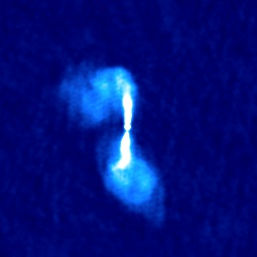
\includegraphics[width=\textwidth]{images/3C_272.1.jpg}
                \caption{M84/3C 272.1}
                \label{fig:m84}
            \end{subfigure}
            \begin{subfigure}{0.45\textwidth}
                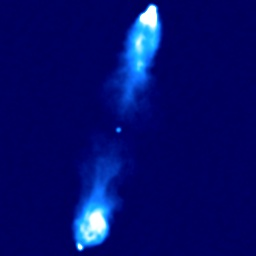
\includegraphics[width=\textwidth]{images/3C_223.jpg}
                \caption{3C 223}
                \label{fig:3C223}
            \end{subfigure}
            \caption[Examples of a FRI and a FRII radio galaxy.]{\label{fig:fri-frii} Examples of (a) a FRI \citep{laing_rotation_1987} and (b) a FRII radio galaxy \citep{leahy_vla_1991}. Both are shown with an arcsinh stretch and were observed with the VLA.}
        \end{figure}

        As powerful sources of radio emission, radio AGN and their associated extended structure can be seen throughout the universe. Sufficiently close or large radio galaxies can be resolved by telescopes and their structure examined, while more distant or smaller radio galaxies may be unresolved and point-like. A well-resolved radio galaxy can be a striking thing: from the central AGN extend two opposing, tightly-collimated jets, which widen into huge lobes of radio-bright plasma. These lobes may have further structure, particularly bright regions called \defn{hot-spots}, and the jets and lobes may be bent and distorted as they travel away from their host galaxy. For any given radio galaxy, some of these features may or may not be present. In particular, radio galaxies are often divided into two classes based on the kinds of extended structure that are visible, called Fanaroff-Riley type I (FRI) and Fanaroff-Riley type II (FRII) radio galaxies. FRI have wavy, diffuse lobes, appearing brighter toward the host galaxy and dimming further out (e.g. \autoref{fig:m84}). FRII, on the other hand, have long, tightly-collimated jets and sharp-edged lobes with bright hot-spots \citep{urry_unified_1995} at the very end of the lobes, and are brighter further away from the host galaxy (e.g. \autoref{fig:3C223}). FRII are also generally higher-luminosity \citep{fanaroff_morphology_1974} than FRI, and therefore make up the majority of observed extended radio sources throughout the universe, but this is by no means the clear-cut divide it was once thought to be \citep{mingo_revisiting_2019} with the difference now being attributed largely to environmental effects rather than jet power. The current understanding is that FRII jets remain at relativistic energies up until the edge of the lobe, where they terminate in a shock that appears as a hot-spot, while FRI jets decelerate within the galaxy itself \citep{hardcastle_radio_2020}, so this sharp difference in extended structure begins with environmental interactions at the very centre of the galaxy.

        A radio galaxy can be tremendously extended, with increasingly many radio galaxies being found with a length of over one megaparsec. Such large galaxies are called \defn{giant radio galaxies}, but even non-giants are still quite big, regularly extending well outside the stellar component of the host galaxy. We will discuss the extended structure in \autoref{sec:extended-structure-of-agn}.

        An AGN interacts with its host galaxy, and so the host galaxy of an AGN can also provide interesting insights into the structure and behaviour of the AGN. Early research indicated that the split between FRI and FRII radio galaxies was dependent on the mid-infrared and optical brightness (and therefore density) of the host galaxy \citep{ledlow_20_1996,bicknell_relativistic_1995} though more recent work suggests this may not be a strong effect if it exists at all \citep{hardcastle_radio_2020}.

    \subsection{Extended structure}
    \label{sec:extended-structure-of-agn}

        The jets and lobes of AGN can be very extended, with the largest known radio galaxies measuring over 4 Mpc end-to-end \citep{machalski_understanding_2011}. This is much larger than the radius of their host galaxies, and so the jets and lobes of AGN are uniquely posed to interact with the local environment. Environmental interactions both within and outside the host galaxy warp and distort the jets and lobes. Within the galaxy, the jets drive a bubble of energy in the interstellar medium \citep[ISM;][]{mukherjee_relativistic_2016}, transferring energy into the ISM with different effects depending on the jet power \citep{mukherjee_relativistic_2018}; the ISM on the other hand suppresses the jets and distorts them to varying amounts depending on the degree of interaction \citep{mukherjee_relativistic_2018}. Outside the galaxy, the jets and lobes are bent by the intra-cluster medium and neighbouring galaxies \citep[ICM;][]{garon_radio_2019, rodman_radio_2019} and this structure may even be used as a probe for cluster environments \citep{banfield_radio_2016,sakelliou_3c40_2008}.

        \begin{figure}
            \centering
            \begin{subfigure}{0.3\textwidth}
                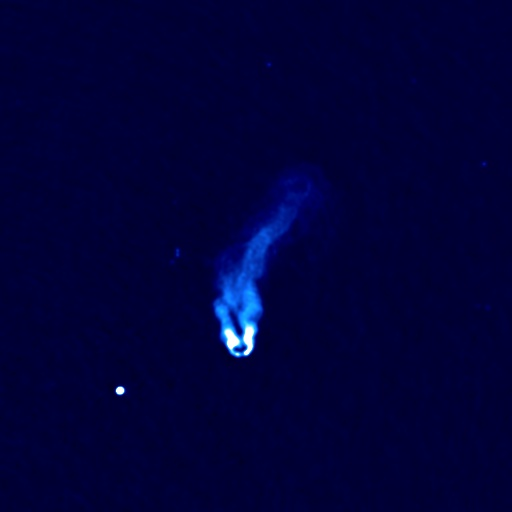
\includegraphics[width=\textwidth]{images/3C_83.1B.jpg}
                \caption{3C 83.1B}
                \label{fig:3C83-1B}
            \end{subfigure}
            \begin{subfigure}{0.3\textwidth}
                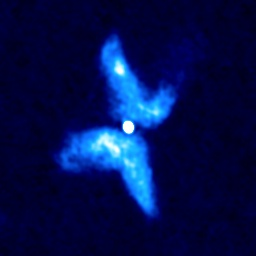
\includegraphics[width=\textwidth]{images/3C_315.jpg}
                \caption{3C 315}
                \label{fig:3C315}
            \end{subfigure}
            \begin{subfigure}{0.3\textwidth}
                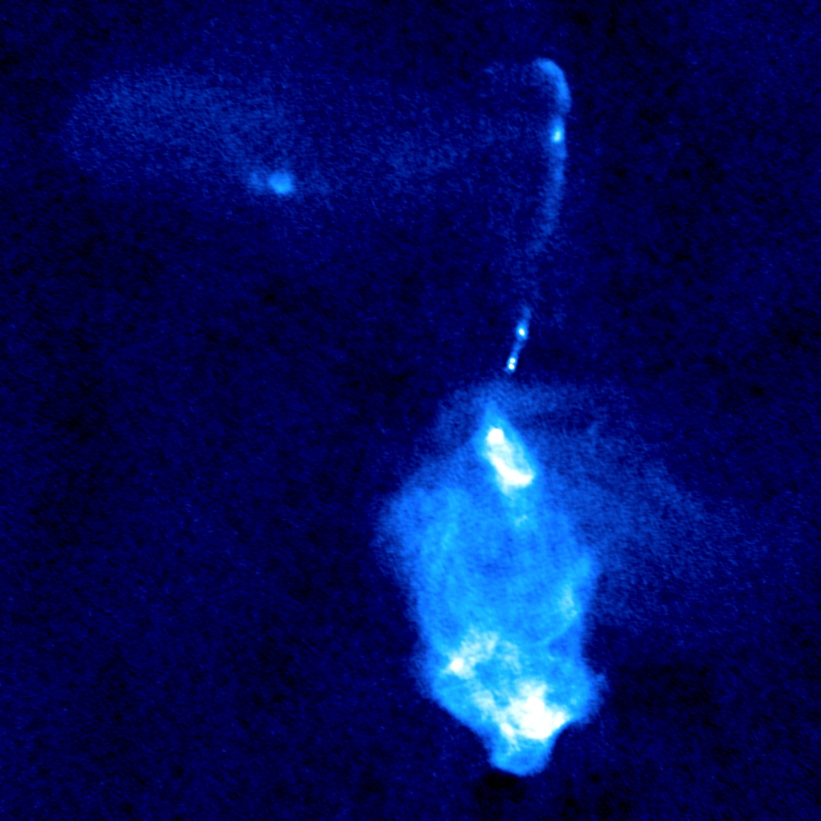
\includegraphics[width=\textwidth]{images/3C_433.jpg}
                \caption{3C 433}
                \label{fig:3C433}
            \end{subfigure}
            \caption[Three radio galaxies with interesting structure.]{Radio galaxies, displayed with an arcsinh colour scale. All images were taken with the VLA. (a) is a narrow-angled tail radio galaxy \citep{leahy_atlas_nodate}, (b) is an X-shaped radio galaxy \citep{leahy_polarization_1986}, and (c) is a very unusually-shaped radio galaxy \citep{black_study_1992}.}
            \label{fig:interesting}
        \end{figure}

        The strong interaction of AGN with their environment leads to a great variety of exotic-shaped radio galaxies. Some morphological classes of this `radio galaxy zoo' include X-shaped galaxies, which have two sets of lobes roughly perpendicular to each other; wide- and narrow-angled tail galaxies, which are bent about the core with large and small angles respectively; head-tail galaxies, which are so bent that the two lobes seem to be the same or nearly the same; double-doubles, which have two sets of lobes on each side; and many, many more. Some examples of radio galaxies with interesting structure are shown in \autoref{fig:interesting}. Large-scale automated identification of these galaxies can be tricky owing to their variety, extent, and often disconnected structure.

        AGN cores tend to have flat or inverted spectral indices around -0.5--1 \citeneeded. Moving out from the host galaxy, the spectral index steepens as the electrons are older and less energetic, with the spectral index of the lobes usually at about -0.7 \citeneeded. The hotspots of FRII galaxies have spectral indices between -0.5 -- -0.7, becoming shallower as the electrons reaccelerate \citeneeded. The jets do not strongly emit and are only detectable for particularly deep observations or nearby radio galaxies \citeneeded.

    \subsection{The unified model}
    \label{sec:unified-model}

        \begin{figure}
            \centering
            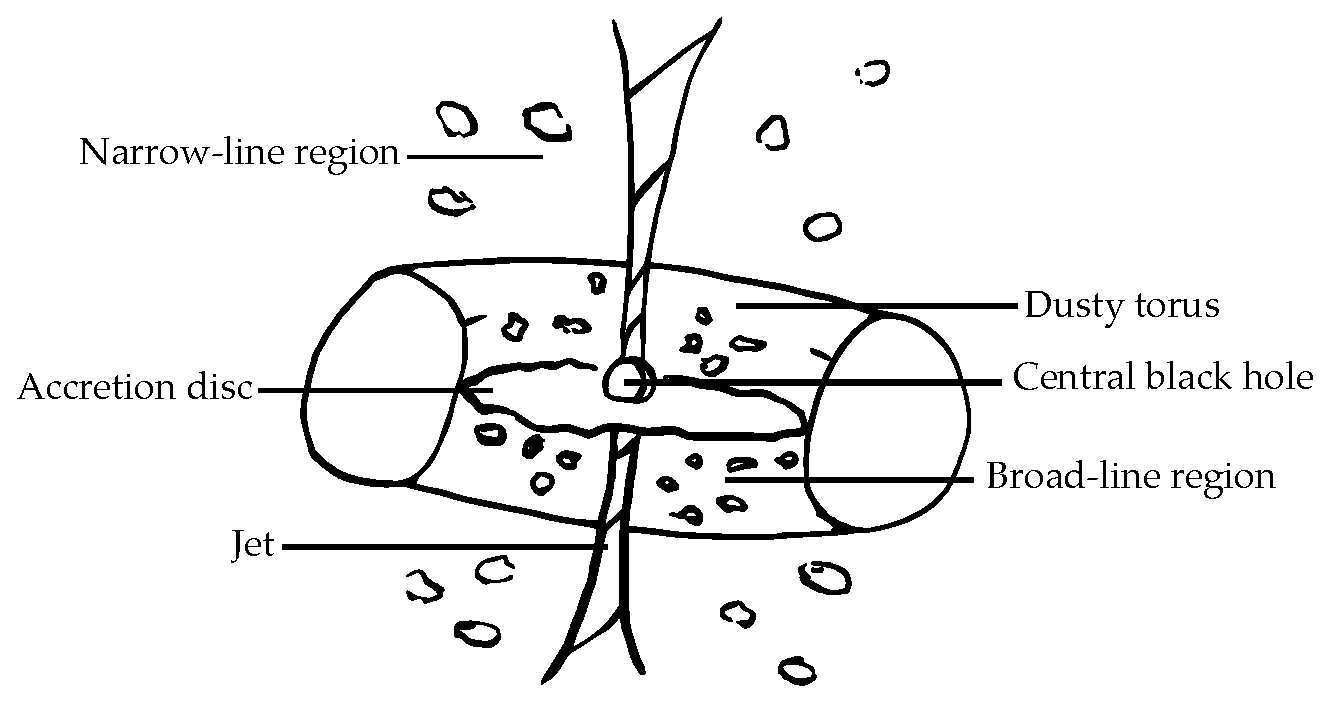
\includegraphics[width=\textwidth]{images/agn.eps}
            \caption{\label{fig:agn} The unified model of AGN.}
        \end{figure}

        At their core, AGN are an accreting \defn{supermassive black hole}: a body so dense that even light cannot escape its gravitational pull, with mass on the order of $10^7$--$10^9\ \mathrm{M}_\odot$ \citeneeded{}. Such black holes seem to exist at the centre of galaxies\citeneeded{} and these galaxies are called \defn{host galaxies}. The current understanding of the structure of an AGN is as follows \citep{urry_unified_1995}. The black hole is surrounded by an accretion disc emitting in ultraviolet and X-ray. Beyond this is the broad-line region, named for the Doppler-broadened emission lines emitted by the energetic clouds of material surrounding the accretion disc. The broad-line region and accretion disc are themselves surrounded by a dusty torus (or some other disc-like structure) which prevents light from the centre of the AGN being observed from the sides. Further still from the accretion disc is the narrow-line region, where lower-energy gas produces narrow emission lines. From either side of the disc, an AGN produces two collimated outflows of relativistic plasma called {jets}, and these jets may interact with gas in the host galaxy to produce bright radio emission. The jets are not always visible. As the jets disperse further out from the centre of the AGN they widen into plumes of plasma known as \defn{lobes}. This model of AGN unifies different observed classes of AGN by their orientation and luminosity, and is hence known as the \defn{unified model} \citep{antonucci_unified_1993}. Recent work suggests that the unified model of AGN is not the full story \citep[e.g.][]{zhuang_interplay_2020}\todo{Explain alternatives to the unified model?}.

        There are many different ways to divide the set of radio AGN into classes. By morphology, radio AGN are often divided by the structure of the jets and lobes, with FRI and FRII the most striking examples. AGN can also be divided into \defn{radiative-mode} and \defn{jet-mode} by how they expel their energy \citep{heckman_coevolution_2014}. Radiative-mode AGN produce radiative energy in amounts higher than 1 percent of their Eddington limit, while jet-mode AGN mainly output energy through their jets. The Eddington limit describes the maximum luminosity that a compact object can emit, and is given in \autoref{eq:eddington} \citep{rybicki_radiative_1979}:
        \begin{equation}
            L_{\mathrm{Eddington}}(M) = \frac{4\pi G M m_p c}{\sigma_T}.
            \label{eq:eddington}
        \end{equation}
        Optical emission observed near the centre of the AGN can be used to divide radio AGN into broad-line and narrow-line galaxies. The former have broad spectral lines while the latter have narrow spectral lines, with broader spectral lines indicative of higher thermal energies. The most common interpretation, under the unified model, is that broad-line AGN are those seen end-on and narrow-line are those seen edge-on with the dusty torus obscuring the broad-line region.\todo{include an alternative explanation} These narrow-line galaxies are usually the only ones for which we see significant extended structure.

    \subsection{Polarised structure}
    \label{sec:polarised-structure-of-agn}

        The magnetic field of AGN is thought to be critical to their structure \citep{sikora_magnetic_2013}. A strong magnetic field is required to eject and collimate the jets \citep{lovelace_dynamo_1976} and the magnetic environment influences the structure of the jets \citep{osullivan_magnetic_2015}. Polarisation provides a probe for measuring this magnetic field. Radiative- and jet- mode AGN have different fractional polarisations, with jet-mode AGN having a much wider range of fractional polarisations ($p \sim [0, 30]$ per cent) compared to radiative-mode AGN (limited to $p \lessapprox 15$ per cent), with this difference attributable to the magnetic environment \citep{osullivan_magnetic_2015}. Steep-spectrum ($\alpha > 0.5$) and flat-spectrum ($\alpha < 0.5$) AGN have differing fractional polarisations, with steep-spectrum sources having much higher fractional polarisation for frequencies $> 5$~GHz and flat-spectrum sources having higher fractional polarisation for frequencies $< 1$~GHz due to frequency-dependent depolarisation of the steep-spectrum sources \citep{saikia_polarization_1988}. Hotspots of FRII radio galaxies have low polarisation ($<10$ per cent) while the more diffuse sections may have much greater polarisation ($>20$ per cent) \citep{saikia_polarization_1988}. The direction of the magnetic field is correlated with the direction of the total intensity of the source \citep{saikia_polarization_1988}. \todo{}

    % \subsection{The host galaxies of AGN}
    % \label{sec:host-galaxies}

    %     This section will discuss the host galaxies of AGN, with necessary reference to their infrared colours as probes of the physics within. How do AGN interact with their host galaxies and vice-versa? \todo{}

    % \subsection{AGN throughout the universe}
    % \label{sec:agn-throughout-the-universe}

    %     What is the expected distribution of AGN? What do simulations say, and what do observations say? Note that AGN get brighter back in time. \todo{}

    \subsection{The role of AGN}
    \label{sec:role-of-agn}

        How do AGN tie into galaxy evolution and feedback? Why do we need them in our models and theories? Why are they important? \todo{}

\section{Classifying AGN}
\label{sec:classification-of-agn}

    As discussed in \autoref{sec:unified-model}, radio galaxies fall into many classes. Understanding the mechanisms underlying these class distinctions is critical to understanding AGN. As we have no way to directly see the core of an AGN (it's far too small to resolve at the distances AGN occur and may also be occluded), our only method to investigate AGN is by looking at their large-scale behaviour. Some classes may relate to the fundamental AGN core, some may be environmental, and some may be due to observation effects. Much of our knowledge about AGN (such as the unified model) come from analysing these classes and their differences. To investigate classes of AGN then a large sample of each class is required, and source classification approaches can divide a large dataset from a radio survey into useful subsets. Knowing what class a source is may also help analyse its properties as we can estimate its expected behaviour, perhaps with the aid of models and simulations. Some classes may have interesting structure or properties that can only be observed with additional detailed observations, so identifying which sources require follow-up is a tightly related problem in radio astronomy. An excellent, though now somewhat dated, summary of radio source classification is the review paper by \citet{urry_unified_1995}, which we recommend for further reading.

    Deciding which class a given radio galaxy falls into may be challenging, and doing this automatically even more so. This section discusses approaches to classifying radio galaxies.

    \subsection{Statistical and manual classification of AGN}
    \label{sec:manual-classification}

        Manual and statistical approaches to classifying AGN have dominated the radio astronomy literature until very recently, due to the comparative lack of computational power as well as a lack of good automated methods. Manual methods amount to examining the structure of a resolved source and determining its class: this is how we usually identify bent radio galaxies, head-tail radio galaxies, X-shaped radio galaxies, and those radio galaxies with more unusual morphologies. Statistical approaches identify properties of the source that can be combined and thresholded to separate the sources into categories en masse. Modern machine learning techniques for classification of radio sources can be thought of as an extension of these statistical methods, where the properties and their combinations are identified automatically, but we will discuss these separately in \autoref{sec:ml-classification-of-agn}.

        Arguably the most well-known radio classification scheme, FRI and FRII, was originally defined on well-resolved radio galaxies by computing the ratio of the distance between the regions of highest brightness on opposite lobes and the total extent of the radio emission \citep{Fanaroff1974}. Sources with a ratio under 0.5 were called FRI and those with a ratio greater than 0.5 were called FRII. This classification has over time evolved into a less precise divide, with classification generally now morphological and based on the structure (diffuse, wavy plumes versus hotspots and lobes for FRI and FRII respectively). The FRI and FRII divide has been further complicated by other related categorisations such as the so-called "Fanaroff-Riley type 0" sources which seem to be the lower end of a continuum of radio sources with diffuse plumes \citep{garofalo_fr0_2019,capetti_lofar_2020}. Many classes are defined by explicitly statistical means; for example, steep- and flat-spectrum sources are divided by spectral index at $\alpha = 0.5$ \citep{urry_unified_1995}. For convenient analysis, radio sources are often also grouped into ``observational'' classes that don't have a physical analogue based on their apparent structure, e.g. the GLEAM survey classifies radio sources into the number of apparent components, which is highly dependent on the observational parameters \citep{white_gleam_2020}.

        More unusual or more loosely defined classes, such as X-shaped radio galaxies and giants, have often been identified by manual searches through large datasets, e.g. \citet{cheung_first_2007,dabhade_search_2020} and notably the recent ROGUE I catalogue of 32~616 morphologically classified radio galaxies \citep{zywucka_catalogue_2020}. These searches are often aided by computer algorithms \citep[e.g.][]{proctor_morphological_2011,dabhade_search_2020}.

        Radio sources are also more generally classified, such as into AGN or non-AGN emission \citep{koziel-wierzbowska_identifying_2020}, often using optical emission lines or optical/infrared magnitude.

    \subsection{Machine learning classification of AGN}
    \label{sec:ml-classification-of-agn}

        Machine learning based approaches for radio source classification are rapidly evolving as the amount of radio data available through big surveys increases. Advances in tooling, such as the wide availability of hardware-accelerated automatic differentiation software, have also contributed to an explosion in machine learning applications in astronomy by making machine learning techniques more available to astronomy researchers.

        Morphological classification of galaxies with machine learning began in optical astronomy, probably due to the large sample sizes of well-resolved galaxies previously available. The earliest such paper is likely the application of neural networks to the task by \citeauthor{storrie-lombardi_morphological_1992} in 1992. From here, the field applied other classification algorithms such as decision trees \citep[e.g.][]{owens_using_1996}. The Sloan Digital Sky Survey (SDSS) brought an explosion of new data in 2003, and new experiments in classification soon followed \citep[e.g.][]{ball_galaxy_2004,ball_robust_2006}. The Galaxy Zoo project leveraged hundreds of thousands of volunteers to produce an astonishingly large set of labelled optical galaxies from SDSS and subsequent papers used this as a training set for machine learning methods \citep{banerji_galaxy_2010,dieleman15cnn,zhu_galaxy_2019}.

        While machine learning has been used in radio astronomy for some time \citep[e.g. the NVSS used neural networks to detect sidelobes;][]{condon_nrao_1998} its first application to radio source classification was most likely to identifying quasar candidates in FIRST \citep{carballo_selection_2004}. \citet{proctor06} applied decision tree ensembles to identify bent double morphologies in FIRST, manually selecting features to characterise radio sources, while \citet{bastien_classifying_2017} used shapelet analysis to obtain features to feed into their decision tree ensembles. 2011--12 marked a revolution in computer vision with the discovery that deep convolutional neural networks \citep[known as early as 1989, see][]{lecun_backpropagation_1989}, boosted dramatically by widely available training data generated by the internet and a huge increase in computational power from GPUs, could achieve greater-than-human performance on image classification tasks. Deep neural networks have since found use for morphological classification of radio sources, such as FRI vs FRII \parencites{aniyan17cnn,ma_machine_2019,lukic_morphological_2019,tang_transfer_2019,samudre_data-efficient_2020,bowles_attention-gating_2020}[see also][]{ma_radio_2018}, compact vs extended sources \citep{lukic18compact,alhassan_first_2018,lukic_morphological_2019}, and observational classes \citep{galvin_radio_2019}.

        There are also many works on classification of radio sources besides morphology. Machine learning has been applied to AGN classification tasks including blazar classification \citep{arsioli_machine_2020} and radio loudness \citep{beaklini_agn_2020}. Deep learning is also prevalent on this topic, with deep learning finding applications in Faraday complexity classification \citep{brown_classifying_2018} and notably in transient detection \citep{connor_applying_2018,guo_pulsar_2019,wang_pulsar_2019,agarwal_fetch_2020,lin_pulsar_2020,zhang_applying_2020,balakrishnan_pulsar_2020}.

        It is worth contrasting these machine learning approaches with non-machine learning automated approaches, as the two are often conflated in the literature. \citet{mingo_revisiting_2019}, for example, use an automated version of detecting the brightness gradient of extended radio sources to determine whether they are FRI or FRII en masse and apply this approach to the LoTSS survey. \citet{segal_identifying_2019} apply an information theoretic approach to estimating morphological complexity of a source. The key difference between a machine learning automated approach and a non-machine learning automated approach is that the former has the capacity to change its behaviour based on available data, while the latter does not --- though note that this is not necessarily a bad thing.

\section{Aggregating Radio Sources}
\label{sec:aggregation}
    
    Unlike galaxies observed at other wavelengths, the emission from radio galaxies can be disconnected when observed: a single radio galaxy may appear in observations as multiple discrete components. This is partly due to inhomogeneous emission over the radio galaxy structure --- e.g. FRII hotspots can be much brighter than the rest of the galaxy, so they might be visible while the rest of the galaxy is too faint to see --- and partly due to the technique through which many radio observations are made, \defn{interferometry}, which may screen out diffuse emission. Since radio galaxies can appear disconnected, aggregating observed radio objects into physical sources is integral to understanding radio galaxies.
    
    \subsection{Missing emission in radio observations}
    \label{sec:missing-emission}

        \begin{figure}
            \centering
            \begin{subfigure}{0.45\textwidth}
                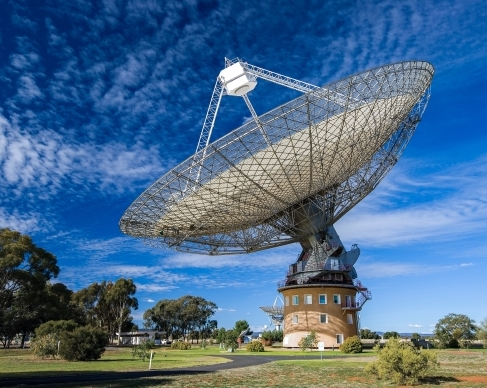
\includegraphics[width=\textwidth]{images/CSIRO-Parkes-Wiradjuri-naming-Murriyang.jpg}
                \caption{The 64m telescope (Murriyang) at Parkes Observatory}
                \label{fig:murriyang}
            \end{subfigure}
            \begin{subfigure}{0.45\textwidth}
                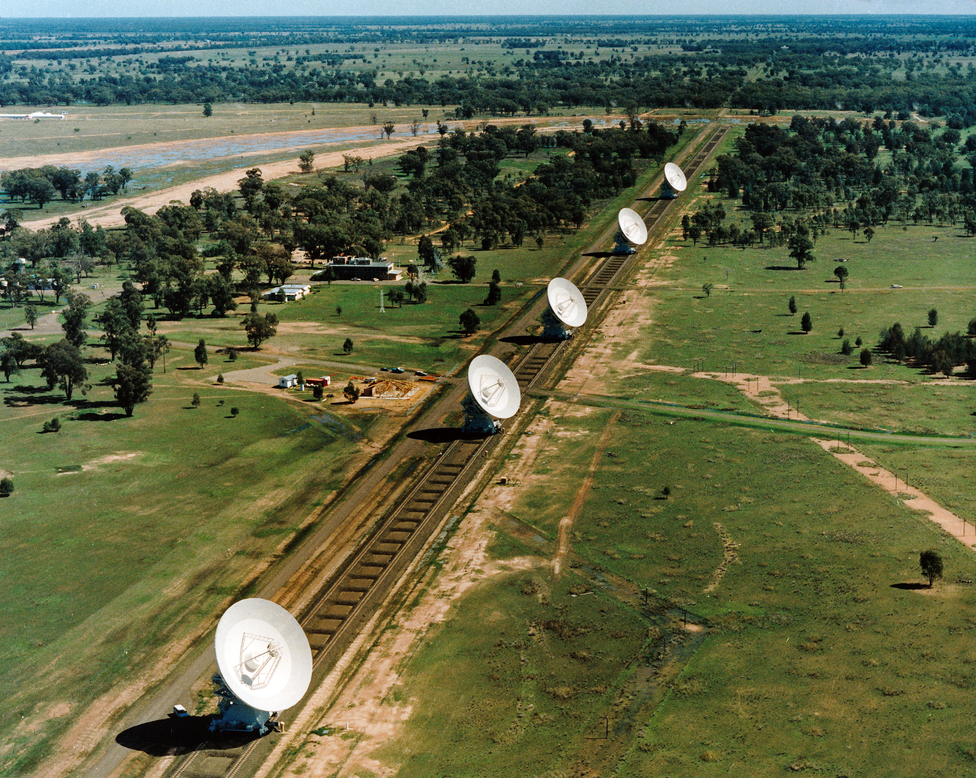
\includegraphics[width=\textwidth]{images/atca.jpg}
                \caption{ATCA near Narrabri}
                \label{fig:atca}
            \end{subfigure}
            \caption[A single dish telescope and a radio array.]{\label{fig:telescopes} (a) A single-dish telescope and (b) an array. Images: CSIRO.}
        \end{figure}

        Radio observations may be made either with \defn{single-dish telescopes}, like the famous Parkes Radio Telescope (Murriyang), or \defn{radio arrays}, like the Australia Telescope Compact Array (ATCA), both shown in \autoref{fig:telescopes}. Both have their advantages. Single-dish telescopes are able to measure absolute brightnesses (while arrays can only measure relative brightnesses, and must therefore be calibrated to a source of known brightness). Interferometric arrays can achieve incredibly high resolution, as the resolution is inversely proportional to the distance between the most distant array elements (while the resolution of single dish telescopes is inversely proportional to the diameter of the dish).

        Radio telescopes can be thought of as sampling the \defn{$u$-$v$ plane}, the Fourier transform of the sky. The $u$-$v$ plane is perpendicular to the line-of-sight. Each pair of antennae in an array samples two points on this plane, each corresponding to the vector between the antennae projected onto the $u$-$v$ plane, called a \defn{baseline}. Longer baselines therefore correspond to higher (spatial) frequencies, which is why long baselines provide high resolution. Diffuse emission is characterised mainly by low (spatial) frequency components, while compact emission is characterised by a broad range of frequency components, so diffuse emission both a) takes up less space on the $u$-$v$ plane than compact sources and b) occupies spaces much closer to the origin on the $u$-$v$ plane. Some intuition on this can be obtained by examining the Fourier transform of a 2D Gaussian:
        \begin{equation}
            \mathcal F_{x, y}\left[\frac{1}{2\pi\sigma^2} e^{-(x^2 + y^2) / 2\sigma^2}\right] = e^{-2\sigma^2 \pi^2(u^2 + v^2)}.
        \end{equation}
        From this equation we can see that the Fourier transform of a fairly \emph{compact} Gaussian would be quite broad, taking up many frequencies in the $u$-$v$ plane, while a very \emph{diffuse} Gaussian would have a very narrow Fourier transform. The upshot of this is that long baselines sacrifice sensitivity to diffuse emission for high resolution. Single-dish radio telescopes are unable to make the same tradeoff, as they are only able to sample a disc centred on the origin\footnote{This is, incidentally, why single-dish telescopes can measure the absolute brightness while arrays cannot: there is no way to measure the origin in the $u$-$v$ plane as there is no way for two array antennae to be infinitely close together (forming a zero-length baseline), and the origin contains the absolute brightness information much like how the centre of a Fourier transform contains the mean.}. This loss of diffuse emission is often called \defn{resolving out}. An example of this is shown in \autoref{fig:resolved-out}, where (a) and (b) are the same radio galaxy observed with the same telescope, the Very Large Array, with the only difference being that the VLA was in B configuration for (a) and the D configuration for (b). The B configuration moves the antennae of the VLA far apart, while the D configuration keeps them close together.

        \begin{figure}
            \centering
            \begin{subfigure}{0.45\textwidth}
                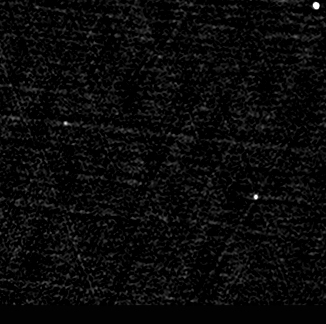
\includegraphics[width=\textwidth]{images/im-contours.jpg}
                \caption{FIRST \citep{becker95first}}
                \label{fig:im-contours-first}
            \end{subfigure}
            \begin{subfigure}{0.45\textwidth}
                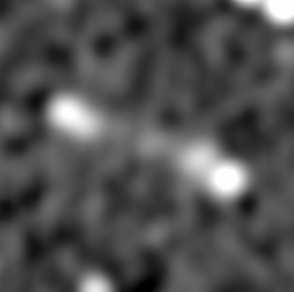
\includegraphics[width=\textwidth]{images/im-contours-2.jpg}
                \caption{NVSS \citep{condon98nvss}}
                \label{fig:im-contours-nvss}
            \end{subfigure}
            \caption[An example of a `resolved out' radio galaxy.]{\label{fig:resolved-out} A fairly diffuse FRII, J0016+0420, observed with the VLA in the (a) FIRST and (b) NVSS surveys. \citep[GRG1 from ][]{dabhade_discovery_2017}}
        \end{figure}

    \subsection{The need to aggregate}
    \label{sec:aggregate-why}

    \subsection{Methods of aggregation}

% \section{Observing Radio Sources}
% \label{sec:radio-astronomy}

% This section needs to talk about how the physics of AGN affects observations and what kind of data we deal with. I'll need to talk about radio telescopes, Fourier transforms, and the noise properties of radio sources, as well as what kind of sources we expect to find throughout the universe. How do observations limit our understanding of AGN? How do observational effects change what we see? What are the main difficulties in radio astronomy?

%     \begin{itemize}
%         \item observational limitations due to physics: \begin{itemize}
%             \item Malmquist bias
%             \item minimum detectable brightness
%             \item minimum detectable physical extent?
%         \end{itemize}
%         \item observing radio: \begin{itemize}
%             \item single-dish radio telescopes (just quickly on this)
%             \item radio arrays
%             \item observations happen in Fourier space
%             \item `resolving out'
%             \item structured noise
%         \end{itemize}
%         \item radio telescopes and radio surveys: \begin{itemize}
%             \item historically
%             \item the NVSS and FIRST
%             \item POSSUM, EMU, RACS
%         \end{itemize}
%     \end{itemize}
